\documentclass[11pt, fleqn]{article}

\usepackage[usenames,dvipsnames,svgnames,table]{xcolor}
\usepackage{amsmath}
\usepackage{amsfonts}
\usepackage[margin=1in]{geometry} % To set the margin widths
\usepackage{graphicx}
\usepackage{listings}
\usepackage{multirow}
\usepackage{tabularx}
\usepackage{varioref}
\usepackage[noabbrev,capitalize]{cleveref}
\usepackage[group-separator={,}]{siunitx}
\usepackage{subcaption}
\usepackage{titlesec}
\usepackage{lscape}
\usepackage{bm}
\usepackage[titletoc,toc,title]{appendix}

\lstset{
  frame=single,
  basicstyle=\ttfamily,% print whole listing small
  language=R,
  aboveskip=3mm,
  belowskip=3mm,
  showstringspaces=false,
  columns=flexible,
  numbers=none,
  commentstyle=\color{ForestGreen},
  stringstyle=\color{Maroon},
  breaklines=true,
  breakatwhitespace=true,
  tabsize=2,
  literate={<-}{{$\gets$}}1 {~}{{$\sim$}}1
}

\sisetup{output-exponent-marker=\textsc{e}}

\setlength{\parskip}{12pt} % Sets a blank line in between paragraphs
\setlength\parindent{0pt} % Sets the indent for each paragraph to zero

\begin{document}

\title{Machine Learning (41204-01)\\HW \#5}
\author{Will Clark $\vert$ Matthew DeLio \\
\texttt{will.clark@chicagobooth.edu} $\vert$ \texttt{mdelio@chicagobooth.edu} \\
University of Chicago Booth School of Business}
\date{\today}
\maketitle

\section{Baseline Predictive Models} \label{baseline}

We use a multinomial logistic regression, a random forest, and a boosting tree as a set of baseline models/algorithms against which we can assess the performance of the neural networks discussed in \cref{nnets}. 

First, we use a multinomial logistic regression model an L1 penalty for variable selection/reduction. We use five-fold cross validation to select the optimal regularization parameter for each classification (i.e. there are six logistic regression models, each with its own L1 penalty). On our test data set, we find that this model predicts movement type with 95.4 percent accuracy. 

Next, we try a random forest algorithm. The only parameter to tune for a random forest is the number of covariates sampled at each tree split (\texttt{mtry}). A rule of thumb is to set $\texttt{mtry}=\sqrt{p}$. In this case, $p=477$, so we estimated a random forest for each of $\texttt{mtry}\in(10, 15, 20, 25, 30)$ so that the range would be roughly centered around $\sqrt{p}$. Again using five-fold cross validation, we found the optimal \texttt{mtry} to be 10. This model predicts out of sample with 94.0 percent accuracy, making it slightly less effective than our multinomial logit model above.\footnote{In sample accuracy was above 98 percent, although the training and test set are composed of different groups of people, so we should not be surprised to see lower OOS accuracy.}

Lastly, we try a boosting tree algorithm. The parameters we can use to tune and the ranges over which we sampled are:
\begin{itemize}
\item \texttt{interaction.depth} $\in (1, 5, 9)$
\item \texttt{n.trees} $\in (500, 1000, 1500, 2000)$
\item \texttt{shrinkage} $\in (0.01, 0.05)$
\end{itemize}
The optimal algorithm, again chosen by five-fold cross validation, used $\texttt{n.trees}=2000$, $\texttt{interaction.depth}=5$, and $\texttt{shrinkage}=0.05$. This algorithm predicts out of sample with 94.4 percent accuracy, making it slightly more accurate than the random forest but still not as accurate as our multinomial logit model.

\begin{landscape}
\begin{figure}
  \centering
  \begin{subfigure}[b]{0.45\textwidth}
    \caption{Lift Plot for Logit Models}
    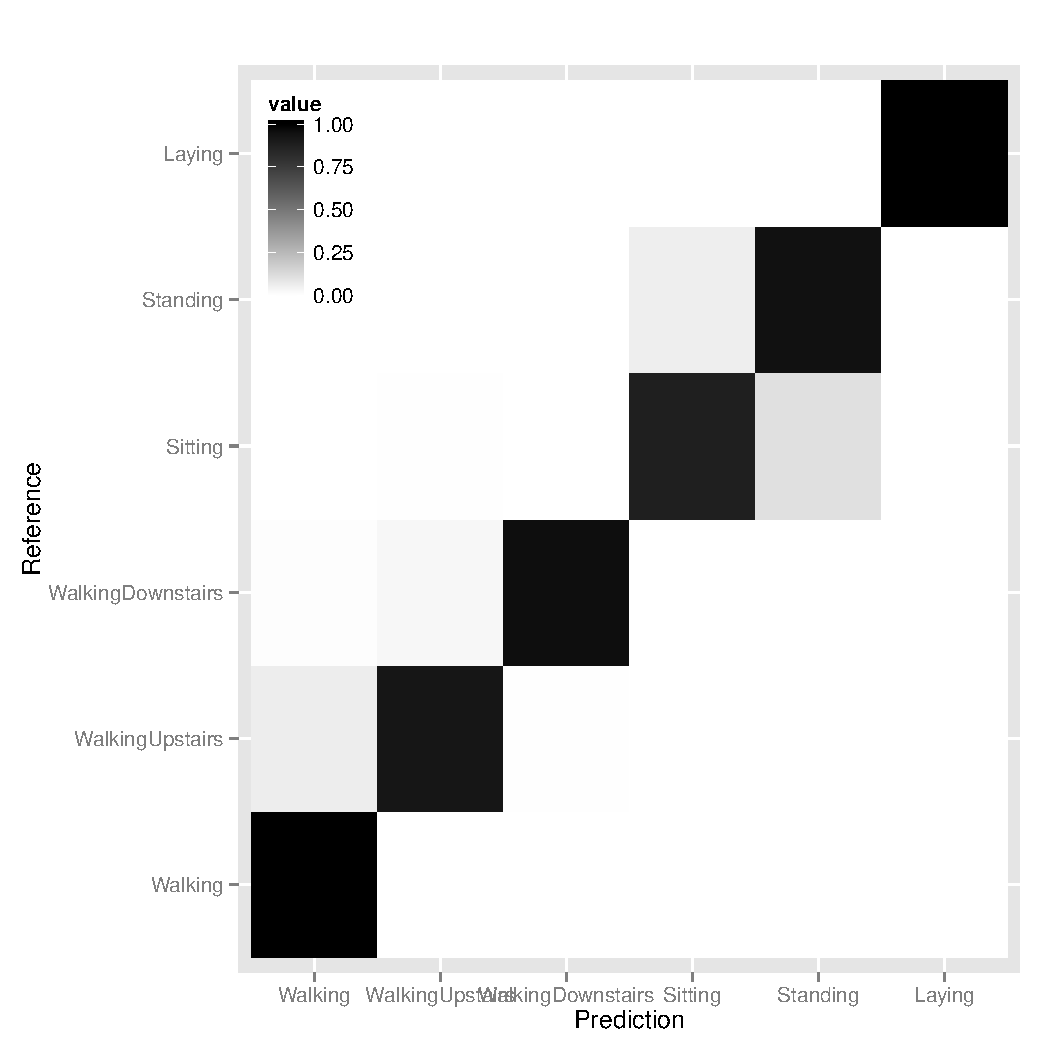
\includegraphics[width=\textwidth]{heatmap_dmr.pdf}
    \label{fig:lift_lin}
  \end{subfigure}
  \hfill
  \begin{subfigure}[b]{0.45\textwidth}
    \caption{Lift Plot for Random Forest}
    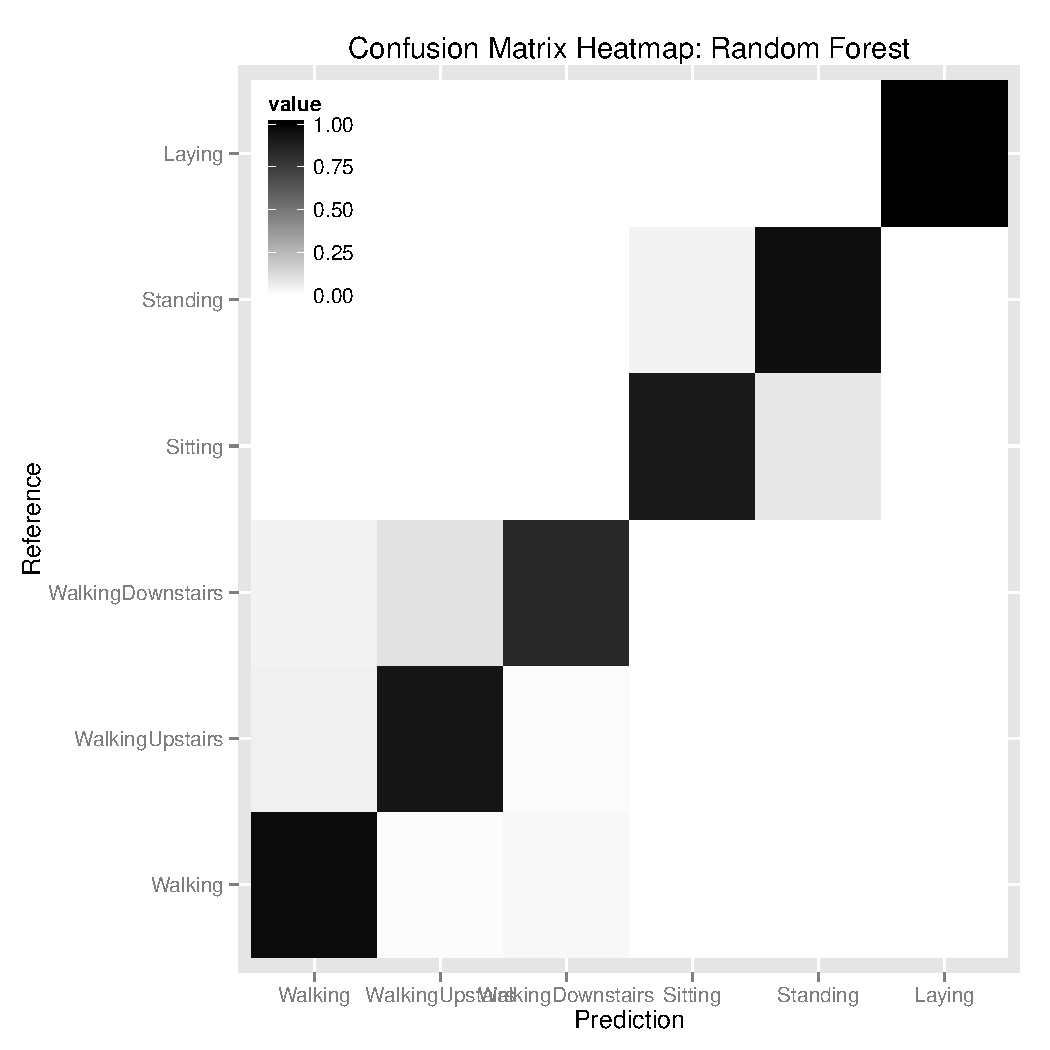
\includegraphics[width=\textwidth]{heatmap_rf.pdf}
    \label{fig:lift_rf}
  \end{subfigure}
  \hfill
    \begin{subfigure}[b]{0.45\textwidth}
    \caption{Lift Plot for Boosting Tree}
    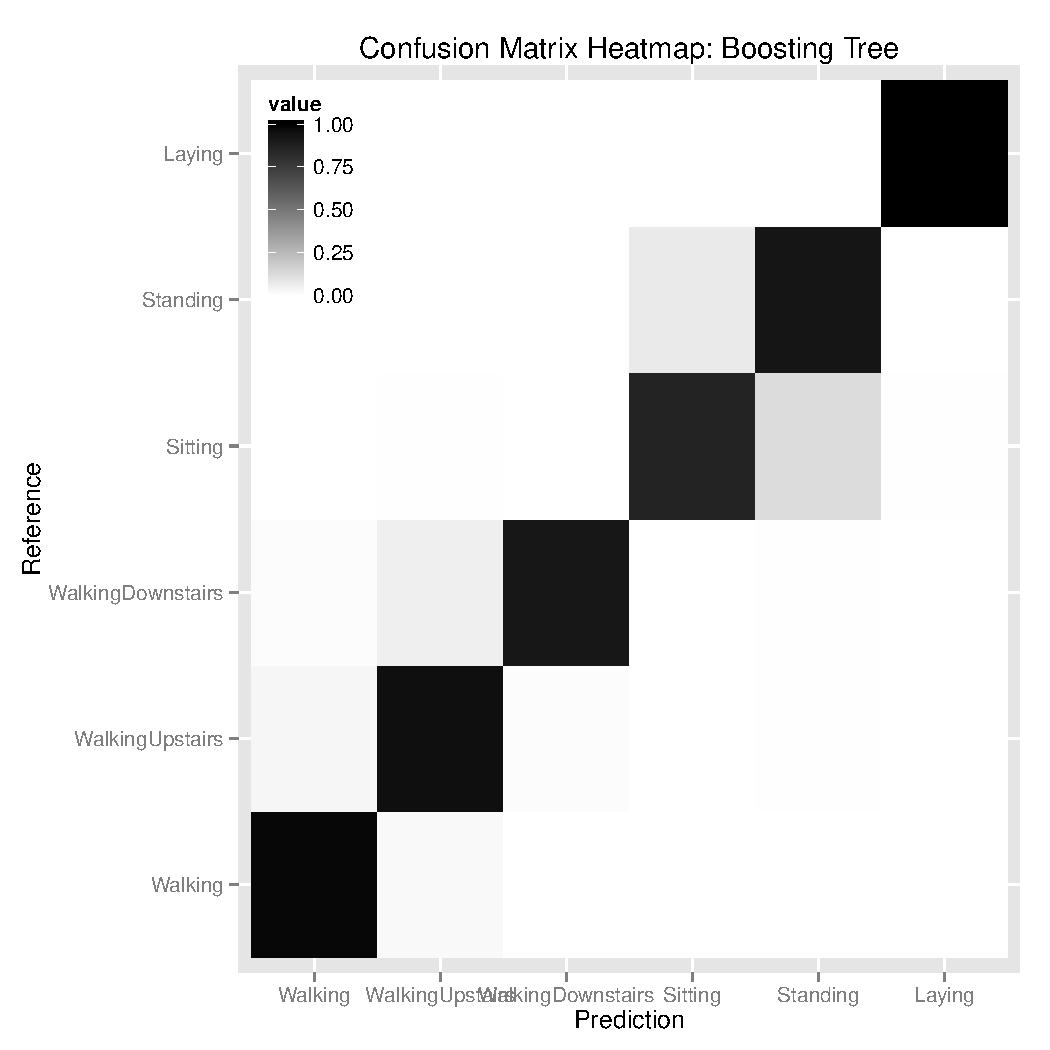
\includegraphics[width=\textwidth]{heatmap_boost.pdf}
    \label{fig:lift_boost}
  \end{subfigure}
  \caption{Lift Plots for Small and Large Models}
\end{figure}
\end{landscape}


\section{Neural Nets} \label{nnets}

% latex table generated in R 3.2.1 by xtable 1.7-4 package
% Wed Nov  4 23:28:56 2015
\begin{table}[ht]
\centering
\caption{Confusion Matrix for Neural Network} 
\label{tab:nnet}
\begin{tabular}{l|rrrrrr}
  &\multicolumn{6}{c}{Reference}\\
 \hline
Predicted & Walking & WalkingUpstairs & WalkingDownstairs & Sitting & Standing & Laying \\ 
  \hline
Walking & 492 &  18 &   4 &   0 &   0 &   0 \\ 
  WalkingUpstairs &   0 & 430 &  14 &   0 &   0 &   0 \\ 
  WalkingDownstairs &   4 &  22 & 402 &   0 &   0 &   0 \\ 
  Sitting &   0 &   0 &   0 & 430 &  60 &   0 \\ 
  Standing &   0 &   1 &   0 &  58 & 472 &   0 \\ 
  Laying &   0 &   0 &   0 &   3 &   0 & 537 \\ 
   \hline
\end{tabular}
\end{table}



\clearpage
\begin{appendices}
\section{Code Listings}
\lstinputlisting[label=lst:code, caption=Code Snippet, language=R]{../hw5.R}
\end{appendices}

\end{document}

% \input{.tex}

% \begin{figure}
%   \centering
%   \begin{subfigure}[b]{0.49\textwidth}
%     \caption{}
%     \includegraphics[width=\textwidth]{.pdf}
%     \label{fig:}
%   \end{subfigure}
%   \hfill
%   \begin{subfigure}[b]{0.49\textwidth}
%     \caption{}
%     \includegraphics[width=\textwidth]{.pdf}
%     \label{fig:}
%   \end{subfigure}
%   \caption{}
% \end{figure}

% \begin{figure}[!htb]
%   \centering
%   \caption{}
%   \includegraphics[scale=.5]{.pdf}
%   \label{fig:}
% \end{figure}

